\def\SetClass{article}
\documentclass{\SetClass}
\usepackage{graphicx} %插入图片的宏包
\usepackage{float} %设置图片浮动位置的宏包
\usepackage{subfigure} %插入多图时用子图显示的宏包
\usepackage[UTF8]{ctex}
\usepackage{geometry} %设置页边距的宏包
\geometry{left=3.0cm,right=2.5cm,top=2.0cm,bottom=2.0cm} %设置页边距
\title{OBOE PAPER SUMMARY}
\author{Ziyu Zhong}

\begin{document}

    \maketitle
    
    \section*{1 思维导图}
    \begin{figure}[!h]
        %是可选项 h表示的是here在这里插入,t表示的是在页面的顶部插入
        \centering
        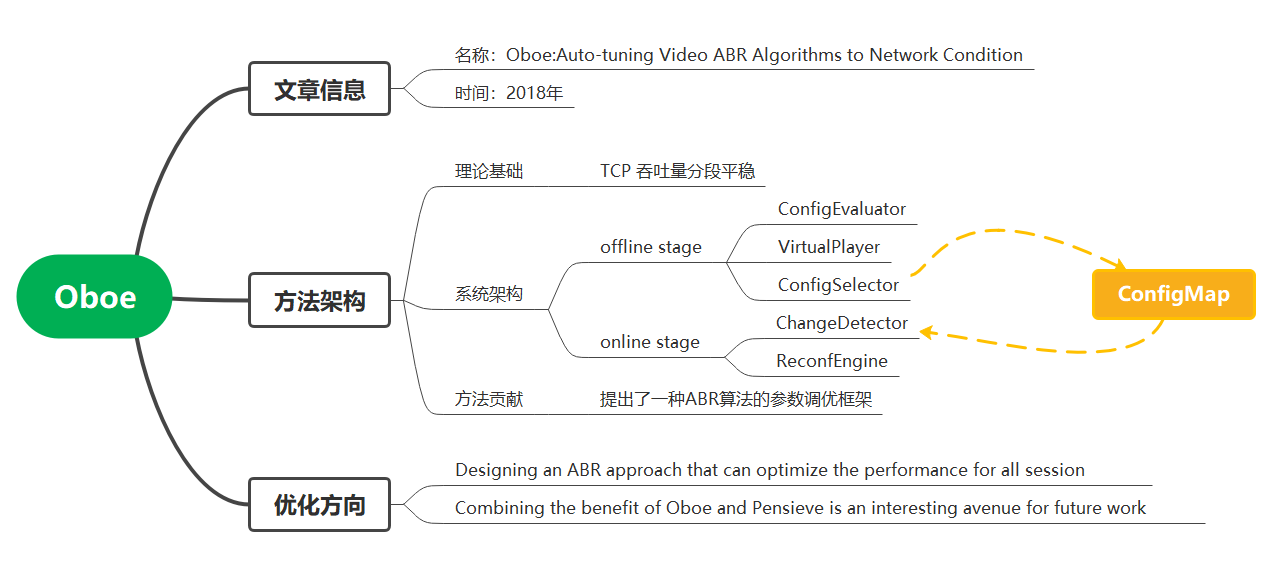
\includegraphics[scale=0.6]{./Fig/mindmap-oboe.png}
        \caption{思维导图}
        \label{fig:1}
    \end{figure}

    \section*{2 文章逻辑}
    \subsection*{2.1 文章信息}
    \begin{itemize}
        \item 名称: Oboe:Auto-tuning Video ABR Algorithms to Network Conditions
        \item 作者: 
        \item 日期: 2018年 
    \end{itemize}
    \subsection*{2.2 提出的问题}
    \par ABR Algorithms have limited dynamic range: they do not perform uniformly well across the range
    of network conditions seen in practice because their parameters are sensitive to throughput variability
    \par 也就是说当前的众多自适应码率算法因为其参数对网络吞吐量敏感,所以并不能在各种网络条件下都表现最优。
    这也表明了在当前方法下,算法性能仍然存在提升空间。同时作者也通过对以往方法实验,说明了参数选取对性能有很大的影响。   

    \subsection*{2.3 提出的方法}
    \subsubsection*{2.3.1 前置条件}
    
    \par TCP connections are well-modeled as traversing a piecewise-stationary sequence of network states:
    the connection consists of multiple non-overlapping segments where each segment is in a distinct stationary 
    network state, where each segment is stationary and often lasts for tens of seconds or minutes.Moreover,the
    throughput in each segment may be modeled as an i.i.d process.
    \par More recent work also shows that TCP throughput is well modeled as a Markov process,each of whose states
    may be modeled as a Gaussion distribution.
    \par 作者对于Oboe的设计是基于前人对于TCP连接建模的研究结论,也就是TCP连接可以分成多段不重叠的独立平稳的网络状态,
    这样我们就可以通过每个分段的统计特征去寻找当前算法下的最优参数。这也是这种方法能获得性能增益的理论基础。
    \par 由于每个TCP连接分片可以建模成独立同分布的高斯过程, 我们可以使用<$\mu_s$,$\sigma_s$>
    对状态建模。

    \subsubsection*{2.3.2 方法架构}

    \par Oboe pre-computes,offline,the best parameter configuration for a given ABR algorithm.
    it does this by subjecting the algorithm,for each state,todifferent parameter values, and picking the 
    one that results in the best performance.Then,duing video playback, Oboe continuously uses a change-point 
    detection algorithm to detect changes in network state and selects the parameter identified by the offline 
    analysis as best for the current state.Thus,if a video session encounters varing network state duing its
    lifetime,Oboe automatically specializes the ABR parameter to each one.
    \par 总体上看,Oboe的方法架构分为了两个大的阶段,一个是离线阶段(offline stage),另一个是在线阶段(online stage)
    接下来分别说明其工作方式。
    \begin{itemize}

        \item 离线阶段: 如图1所示为Oboe的在线阶段工作示意图
        \begin{figure}[!h]
            %是可选项 h表示的是here在这里插入,t表示的是在页面的顶部插入
            \centering
            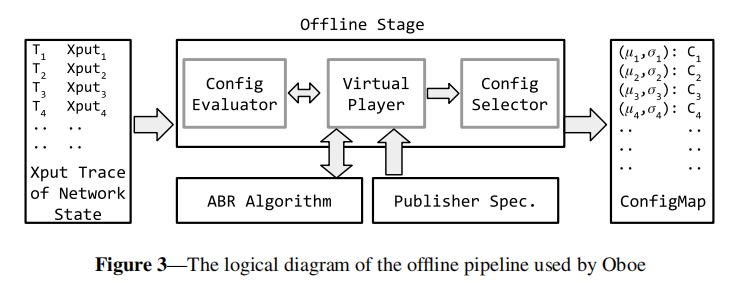
\includegraphics[scale=0.6]{./Fig/offline.png}
            \caption{offline}
            \label{fig:1}
        \end{figure}
        \begin{itemize}
            \item ConfigEvaluator: 从人工合成的trace中提取出$<\mu_s,\sigma_s>$形式的数据(ADF假设试验)。
            
            \item VirtualPlayer: 模拟虚拟的播放场景,省略真实中下载和播放的过程,输入throughput trace,输出QoE metrics。
            将每种配置对应的QoE表现记录下来,给到ConfigSelector。
            
            \item ConfigSelector: 根据从VirtualPlayer拿到的信息,选取每种状态下最佳的配置。
            最终得到网络状态和算法参数对应的ConfigMap。
            
            \item Publisher Spec.: 发布者可以根据自己的偏好来调整QoE的评估方式。
        \end{itemize}


        \item 在线阶段: 如图2所示为Oboe的在线阶段工作示意图
        \begin{figure}[!h]
            %是可选项 h表示的是here在这里插入,t表示的是在页面的顶部插入
            \centering
            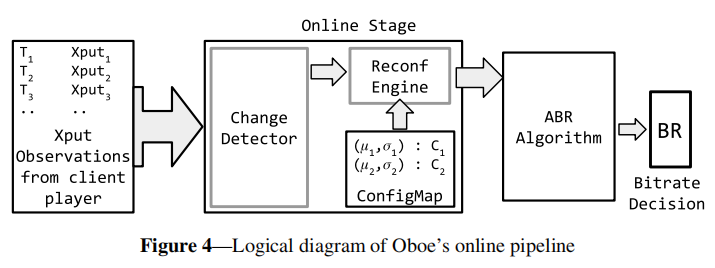
\includegraphics[scale=0.6]{./Fig/online.png}
            \caption{online}
            \label{fig:2}
        \end{figure}
        \begin{itemize}
            \item ChangeDetector: 当观测到throughput trace的统计特性发生明显变化时,马上更新当前网络状态
            
            \item ReconfEngine: 根据新的网络状态$s$,在ConfigMap中以$s$为圆心,$r$为半径选取最保守的策略。
            
        \end{itemize}
    \end{itemize}


    \subsection*{2.4 方法的贡献}
    \par 个人角度理解,本文的方法提出一个通用的ABR算法的优化框架,基于现有的多种方法对参数敏感的特点出发,结合
    前人对于throughput trace统计特性的研究,将某个时间片的throughput的统计特性作为一个状态,基于大量生成的trace模拟
    生成最优“状态-动作”查找表,在应用时再根据查找表作出最优决策。

    \par 和Pensieve对比,两者都针对泛化性能有提升,都有从数据中学习经验的过程。个人觉得不同在于,Pensieve的底层逻辑是强化学习,其基本性能取决于学习算法优劣,
    而Oboe则是一个人工设计的参数选取策略,其性能应该会受制于ABR算法本身的优劣,所以Oboe一定程度上是在榨干已有算法的潜在性能,
    将fixed parameters变为dynamic parameters.
    \subsection*{2.5 可优化的方向}
    \par Online stage deployment? client side or server side better? The detailed comparison of these choices 
    is left to future work. 

    \par Whether Oboe can tune all algorithms and all parameters is an open question. 
    It is also unclear if Oboe can directly augment Pensieve. Combining the benefit of 
    Oboe and Pensieve is an interesting avenue for future work.

    \par As the experiments results shows, Oboe improve most but not all sessions relatice to the
    algorithm it tunes.In some sessions, it meets degration.Generally, designing an ABR approach that
    can optimize the performance for all sessions is a har problem that needs more research.

    \section*{3 遗留的问题}
    \par 在online stage的时候完全是依赖于offline stage生成的ConfigMap进行决策,那么是不是意味着offline在模拟真实场景要
    建模足够准确,那么如何评估建模方式,哪些因素需要考虑,哪些因素可以忽略简化,现在学界是否已经有一个比较通用并验证可靠的建
    模方式。再考虑实际应用中,如果出现了一些新的未知状态,是否就会带来性能的损失,这方面问题是否值得考虑?

    \par 另外还有一点疑问,我们知道ConfigMap是离散的,并且文中已经对trace的state进行了量化大小的测试,得出进一步量化的性能提升并不大。
    而在实际中的trace状态是连续的,所以在实际通过ConfigMap寻找策略时,文中提到了半径$r$为范围选取最保守策略,但似乎没给出定量性的说明,
    比如r的取值范围,以及选最保守是否就对应了当前QoE下的最优选择,也就是说关于这个策略选取是否有继续压榨性能的可能?

    \par 该方法由于ChangeDetector的存在,是否有滞后性问题(没细看)


\end{document}